\chapter{Electromagnetic Induction}

\section{Magnetic Flux and Flux Linkage}

\begin{definition}
    \vocab{Magnetic flux} ($\F$) is the product of an area and the component of the magnetic flux density perpendicular to that area.
\end{definition}

Mathematically, \[\F = B_{\perp} A = BA\cos\t,\] where the magnetic flux density $B$ is at an angle $\t$ to the normal of the area $A$.

The SI unit of magnetic flux is the weber (Wb).

\begin{definition}
    For a coil of $N$ turns, the \vocab{magnetic flux linkage} is defined as the product of the flux $\F$ and the number of turns $N$, i.e. \[\text{magnetic flux linkage} = N\F = NBA\cos\t.\]
\end{definition}

\section{Faraday's Law and Lenz's Law}

Electromagnetic induction refers to the phenomenon that a changing magnetic flux could induce an electromotive force in a conductor.

\begin{law}[Faraday's Law]
    The magnitude of the induced electromotive force in a conductor is proportional to the rate of change of its magnetic flux linkage.
\end{law}

\begin{law}[Lenz's Law]
    The induced current will flow in a direction that produces effects which oppose the change that induced it.
\end{law}

Faraday's law and Lenz's law can be combined to form the equation \[E = -\der{\bp{N\F}}{t}.\]

Note that a current is induced only if there is a complete circuit. An electromotive force is always induced when there is a change in magnetic flux linkage.

\begin{proposition}
    The magnitude of the electromotive force $E$ induced in a wire of length $L$ moving at velocity $v$ in a uniform magnetic field of flux density $B$, with both $L$ and $v$ perpendicular to $B$, is given by \[\abs{E} = \abs{BLv}.\]
\end{proposition}
\begin{proof}
    The area that the wire sweeps out per unit time is given by $Lv$. Thus, \[\abs{E} = \abs{\der{\F}{t}} = \abs{\der{\bp{BA}}{t}} = \abs{B \der{A}{t}} = \abs{BLv}.\] Note that $N = 1$ since we have only a single conductor (the wire).
\end{proof}

The direction of the induced current in the wire, which is perpendicular to both the magnetic field and the motion of the wire, can be predicted using Fleming's right-hand rule: if the thumb and the first two fingers of the right hand are held so that they are mutually at right-angles, then they represent speed ($v$), field ($B$) and current ($I$) respectively.

\section{Applications}

\subsection{Generator}

Electric generators convert mechanical energy into electrical energy.

When a coil of $N$ turns rotates with a constant angular velocity $\o$ in a uniform magnetic field $B$, an electromotive force $E$ is induced.

\begin{figure}[H]
    \centering
    \includegraphics{media/Generator.png}
    \caption{An example of a generator.\protect\footnotemark}
\end{figure}
\footnotetext{Source: \url{https://www.watelectrical.com/electrical-generator-working-types-and-applications/}}

Assume at time $t = 0$, the coil is perpendicular to the magnetic field. Then $\t = \o t$, so the flux linkage through the coil is given by \[N\F = NBA\cos{\o t}.\] From the laws of induction, the induced electromotive force is given by \[E = -\der{\bp{N\F}}{t} = NBA\o \sin{\o t}.\]

\begin{figure}[H]
    \centering
    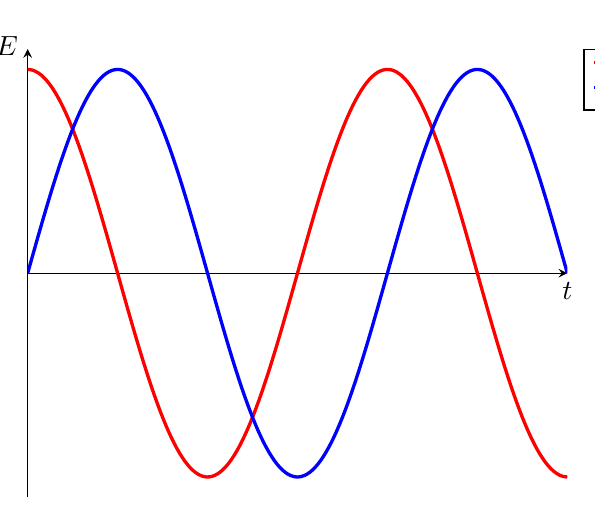
\begin{tikzpicture}[trim axis left, trim axis right]
        \begin{axis}[
            domain=0:3*pi,
            xmax = 3*pi,
            xmin = 0,
            axis y line=middle,
            axis x line=middle,
            samples=200,
            ymax = 1.1,
            ymin = -1.1,
            xtick = \empty,
            ytick = \empty,
            xlabel = {$t$},
            ylabel = {$\F$, $E$},
            legend cell align={left},
            legend pos=outer north east,
            ylabel style = {left},
            xlabel style = {below},
            ]
            
            \addplot[red, very thick] {cos(deg(x))};
            \addlegendentry{$\F$};

            \addplot[blue, very thick] {sin(deg(x))};
            \addlegendentry{$E$};
        \end{axis}
    \end{tikzpicture}
    \caption{A graph of $\F$ and $E$ over time.}
\end{figure}

From this equation, we deduce that
\begin{itemize}
    \item when the flux linking the coil is maximum, the induced electromotive force is zero; and
    \item when the flux linking the coil is zero, the induced electromotive force is maximum.
\end{itemize}

\subsection{Eddy Current}

According to Faraday's law, any relative motion between a conductor and a magnetic field will give rise to an induced electromotive force in the conductor.

If the magnetic field across a conducting body is not uniform, the induced electromotive force in different parts of the body will be different, giving rise to circulating currents within the body, called \vocab{eddy currents}.

According to Lenz's law, the eddy currents will give rise to effects that oppose the relative motion, hence slowing the relative motion. Due to the body's resistance, energy will be dissipated by the eddy currents as thermal energy.